\documentclass[11pt,preprint, authoryear]{elsarticle}

\usepackage{lmodern}
%%%% My spacing
\usepackage{setspace}
\setstretch{1.2}
\DeclareMathSizes{12}{14}{10}{10}

% Wrap around which gives all figures included the [H] command, or places it "here". This can be tedious to code in Rmarkdown.
\usepackage{float}
\let\origfigure\figure
\let\endorigfigure\endfigure
\renewenvironment{figure}[1][2] {
    \expandafter\origfigure\expandafter[H]
} {
    \endorigfigure
}

\let\origtable\table
\let\endorigtable\endtable
\renewenvironment{table}[1][2] {
    \expandafter\origtable\expandafter[H]
} {
    \endorigtable
}


\usepackage{ifxetex,ifluatex}
\usepackage{fixltx2e} % provides \textsubscript
\ifnum 0\ifxetex 1\fi\ifluatex 1\fi=0 % if pdftex
  \usepackage[T1]{fontenc}
  \usepackage[utf8]{inputenc}
\else % if luatex or xelatex
  \ifxetex
    \usepackage{mathspec}
    \usepackage{xltxtra,xunicode}
  \else
    \usepackage{fontspec}
  \fi
  \defaultfontfeatures{Mapping=tex-text,Scale=MatchLowercase}
  \newcommand{\euro}{€}
\fi

\usepackage{amssymb, amsmath, amsthm, amsfonts}

\def\bibsection{\section*{References}} %%% Make "References" appear before bibliography


\usepackage[round]{natbib}

\usepackage{longtable}
\usepackage[margin=2.3cm,bottom=2cm,top=2.5cm, includefoot]{geometry}
\usepackage{fancyhdr}
\usepackage[bottom, hang, flushmargin]{footmisc}
\usepackage{graphicx}
\numberwithin{equation}{section}
\numberwithin{figure}{section}
\numberwithin{table}{section}
\setlength{\parindent}{0cm}
\setlength{\parskip}{1.3ex plus 0.5ex minus 0.3ex}
\usepackage{textcomp}
\renewcommand{\headrulewidth}{0.2pt}
\renewcommand{\footrulewidth}{0.3pt}

\usepackage{array}
\newcolumntype{x}[1]{>{\centering\arraybackslash\hspace{0pt}}p{#1}}

%%%%  Remove the "preprint submitted to" part. Don't worry about this either, it just looks better without it:
\makeatletter
\def\ps@pprintTitle{%
  \let\@oddhead\@empty
  \let\@evenhead\@empty
  \let\@oddfoot\@empty
  \let\@evenfoot\@oddfoot
}
\makeatother

 \def\tightlist{} % This allows for subbullets!

\usepackage{hyperref}
\hypersetup{breaklinks=true,
            bookmarks=true,
            colorlinks=true,
            citecolor=blue,
            urlcolor=blue,
            linkcolor=blue,
            pdfborder={0 0 0}}


% The following packages allow huxtable to work:
\usepackage{siunitx}
\usepackage{multirow}
\usepackage{hhline}
\usepackage{calc}
\usepackage{tabularx}
\usepackage{booktabs}
\usepackage{caption}


\newenvironment{columns}[1][]{}{}

\newenvironment{column}[1]{\begin{minipage}{#1}\ignorespaces}{%
\end{minipage}
\ifhmode\unskip\fi
\aftergroup\useignorespacesandallpars}

\def\useignorespacesandallpars#1\ignorespaces\fi{%
#1\fi\ignorespacesandallpars}

\makeatletter
\def\ignorespacesandallpars{%
  \@ifnextchar\par
    {\expandafter\ignorespacesandallpars\@gobble}%
    {}%
}
\makeatother

\newenvironment{CSLReferences}[2]{%
}

\urlstyle{same}  % don't use monospace font for urls
\setlength{\parindent}{0pt}
\setlength{\parskip}{6pt plus 2pt minus 1pt}
\setlength{\emergencystretch}{3em}  % prevent overfull lines
\setcounter{secnumdepth}{5}

%%% Use protect on footnotes to avoid problems with footnotes in titles
\let\rmarkdownfootnote\footnote%
\def\footnote{\protect\rmarkdownfootnote}
\IfFileExists{upquote.sty}{\usepackage{upquote}}{}

%%% Include extra packages specified by user
\usepackage{booktabs}
\usepackage{caption}
\usepackage{longtable}

%%% Hard setting column skips for reports - this ensures greater consistency and control over the length settings in the document.
%% page layout
%% paragraphs
\setlength{\baselineskip}{12pt plus 0pt minus 0pt}
\setlength{\parskip}{12pt plus 0pt minus 0pt}
\setlength{\parindent}{0pt plus 0pt minus 0pt}
%% floats
\setlength{\floatsep}{12pt plus 0 pt minus 0pt}
\setlength{\textfloatsep}{20pt plus 0pt minus 0pt}
\setlength{\intextsep}{14pt plus 0pt minus 0pt}
\setlength{\dbltextfloatsep}{20pt plus 0pt minus 0pt}
\setlength{\dblfloatsep}{14pt plus 0pt minus 0pt}
%% maths
\setlength{\abovedisplayskip}{12pt plus 0pt minus 0pt}
\setlength{\belowdisplayskip}{12pt plus 0pt minus 0pt}
%% lists
\setlength{\topsep}{10pt plus 0pt minus 0pt}
\setlength{\partopsep}{3pt plus 0pt minus 0pt}
\setlength{\itemsep}{5pt plus 0pt minus 0pt}
\setlength{\labelsep}{8mm plus 0mm minus 0mm}
\setlength{\parsep}{\the\parskip}
\setlength{\listparindent}{\the\parindent}
%% verbatim
\setlength{\fboxsep}{5pt plus 0pt minus 0pt}



\begin{document}



\begin{frontmatter}  %

\title{Question 2: Currency Hedging Analysis}

% Set to FALSE if wanting to remove title (for submission)




\author[Add1]{Jan-Hendrik Pretorius}
\ead{20713479@sun.ac.za}





\address[Add1]{Stellenbosch University}


\begin{abstract}
\small{
This report examines the impact of currency hedging on a 60/40
Equity/Bond portfolio. Comparing hedged and unhedged strategies, we
analyze their effects on portfolio volatility and performance, providing
insights for effective currency risk management in portfolio
construction.
}
\end{abstract}

\vspace{1cm}





\vspace{0.5cm}

\end{frontmatter}

\setcounter{footnote}{0}



%________________________
% Header and Footers
%%%%%%%%%%%%%%%%%%%%%%%%%%%%%%%%%
\pagestyle{fancy}
\chead{}
\rhead{Question 2: Currency Hedging Analysis}
\lfoot{}
\rfoot{\footnotesize Page \thepage}
\lhead{}
%\rfoot{\footnotesize Page \thepage } % "e.g. Page 2"
\cfoot{}

%\setlength\headheight{30pt}
%%%%%%%%%%%%%%%%%%%%%%%%%%%%%%%%%
%________________________

\headsep 35pt % So that header does not go over title




\hypertarget{hedged-vs-unhedged-growth}{%
\section{Hedged vs Unhedged Growth}\label{hedged-vs-unhedged-growth}}

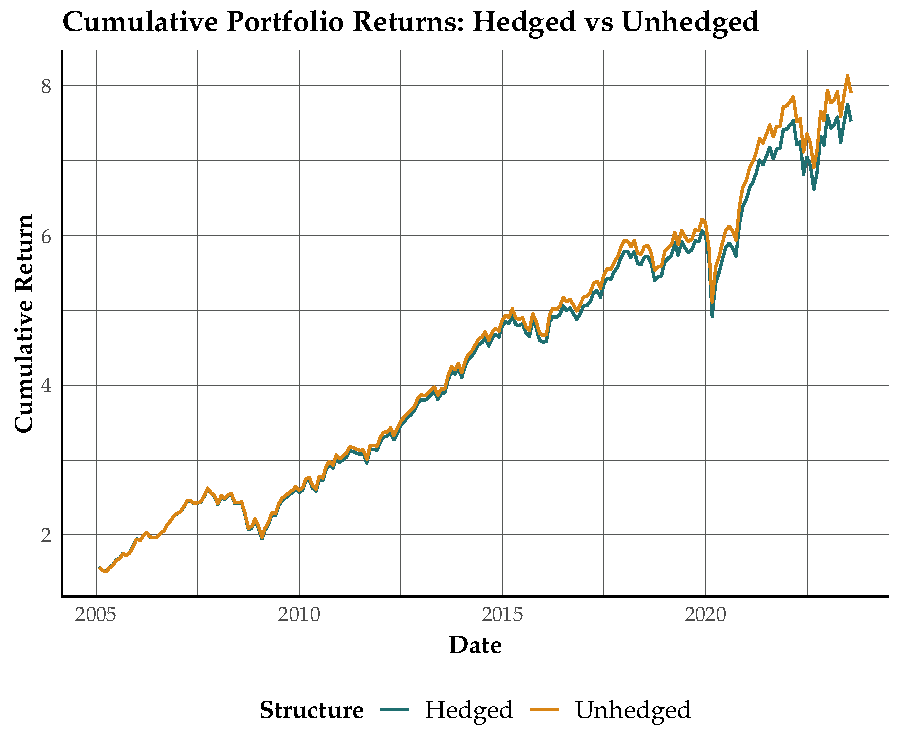
\includegraphics{Question-2_files/figure-latex/cumrets-1.pdf}

The graph above illustrates the cumulative returns of hedged versus
unhedged portfolios from 2005 onwards. Both strategies show growth over
time, with the hedged portfolio occasionally outperforming the unhedged
one. There is some divergence, particularly during periods of market
volatility, but the long-term trajectory of both portfolios appears
similar, indicating that hedging may not significantly impact cumulative
returns over an extended period.

The 3-year rolling returns chart below for hedged and unhedged
portfolios highlights fluctuations over time. Despite some periods where
the hedged portfolio shows slightly lower volatility, overall, both
portfolios follow a similar pattern. This suggests that hedging may not
provide a clear advantage in smoothing returns over a three-year rolling
period.

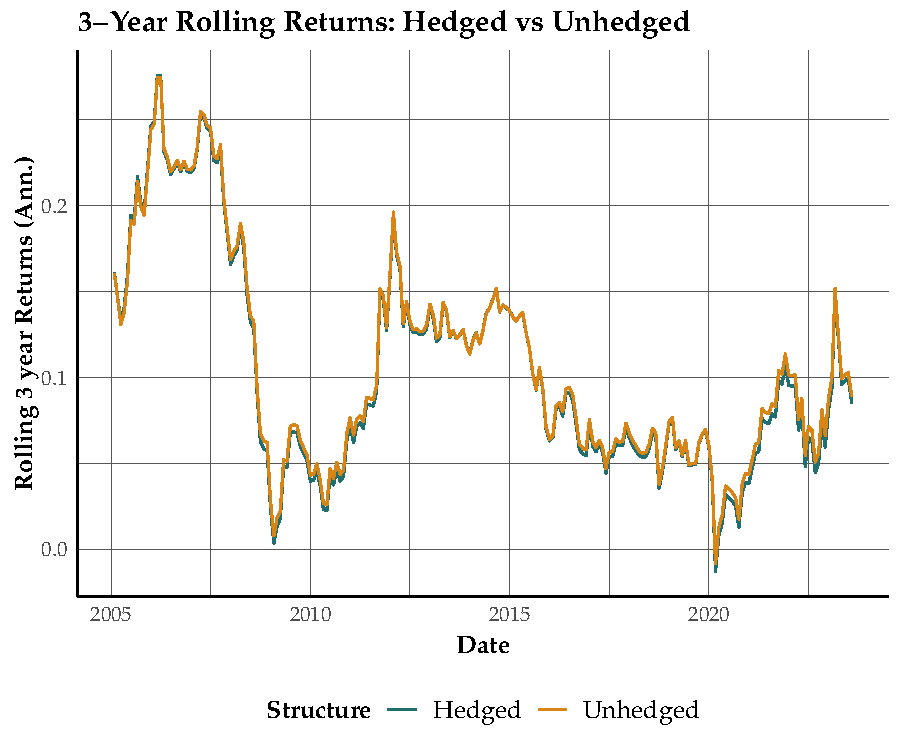
\includegraphics{Question-2_files/figure-latex/rollrets-1.pdf}

The figure below was replicated from a recent study around currency
hedging. It shows how global allocation and the rand have a strong
negative relationship since 2004. This means that when one goes up, the
other goes down, and vice versa. This happens because both are
influenced by the same global factors. For example, when there's
positive risk sentiment, both global allocation and the rand tend to do
well, and when sentiment is negative, they both suffer.

Also, notice that the rand tends to drop more significantly in value in
a month than it appreciates. So, if you make a wrong hedge (on the right
side of the plot), it can be much costlier than the benefit of getting
it right (on the left side).

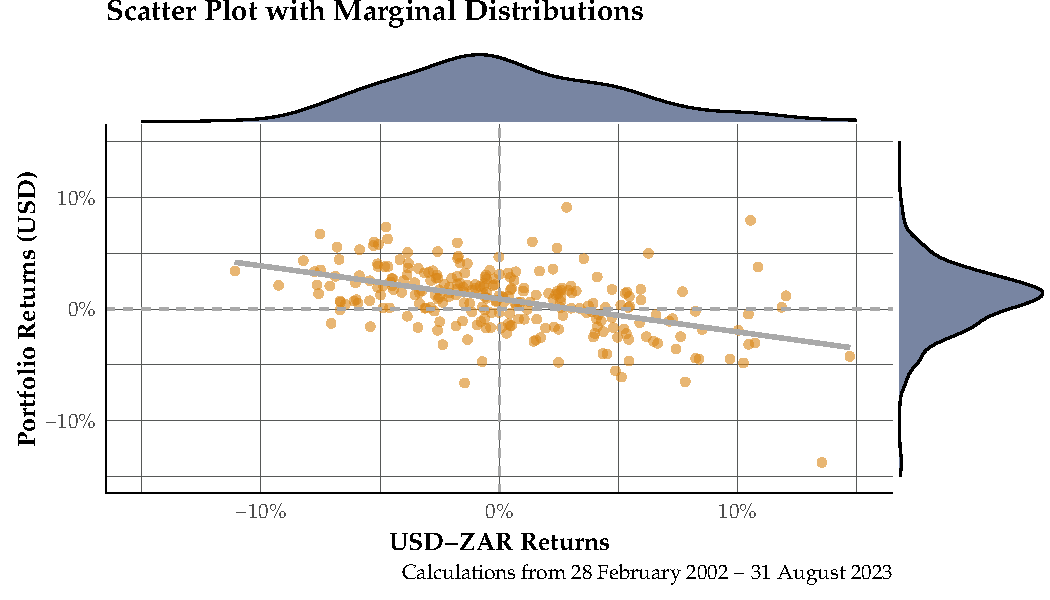
\includegraphics{Question-2_files/figure-latex/scatterplot-1.pdf}

\hypertarget{volatility}{%
\section{Volatility}\label{volatility}}

When comparing the hedged and unhedged portfolios, the hedged portfolio
tends to exhibit slightly higher downside risk, as indicated by the
higher values in semi-deviation, downside deviation, maximum drawdown,
VaR, ES, and modified VaR. However, the differences between the two
portfolios are relatively small, suggesting that the choice between
hedging or not may depend on other factors such as investment goals and
risk tolerance. This information is presented in the table below.

\begin{longtable}{l|rr}
\caption*{
{\large Downside Risk Estimates}
} \\ 
\toprule
\multicolumn{1}{l}{} & Unhedged & Hedged \\ 
\midrule
Semi Deviation & $2.15\%$ & $2.19\%$ \\ 
Downside Deviation (Rf=0\%) & $1.78\%$ & $1.84\%$ \\ 
Maximum Drawdown & $24.96\%$ & $25.65\%$ \\ 
Historical VaR (95\%) & $-4.15\%$ & $-4.22\%$ \\ 
Historical ES (95\%) & $-5.98\%$ & $-6.16\%$ \\ 
Modified VaR (95\%) & $-4.26\%$ & $-4.40\%$ \\ 
Modified ES (95\%) & $-7.03\%$ & $-7.58\%$ \\ 
\bottomrule
\end{longtable}

The graphical representations presented in the following figures (which
include the 36-month rolling volatility, volatility histogram, and
violin plot) provide compelling evidence that hedging strategies may not
deliver the anticipated reduction in volatility. In fact, the data
suggests a counterintuitive trend---over extended timeframes, volatility
tends to exhibit an upward trajectory. This unexpected pattern
challenges the fundamental goal of hedging, which is often implemented
to mitigate risk and stabilize portfolio performance. This intriguing
finding invites further exploration and analysis into the dynamics of
hedging and its long-term impact on portfolio volatility.

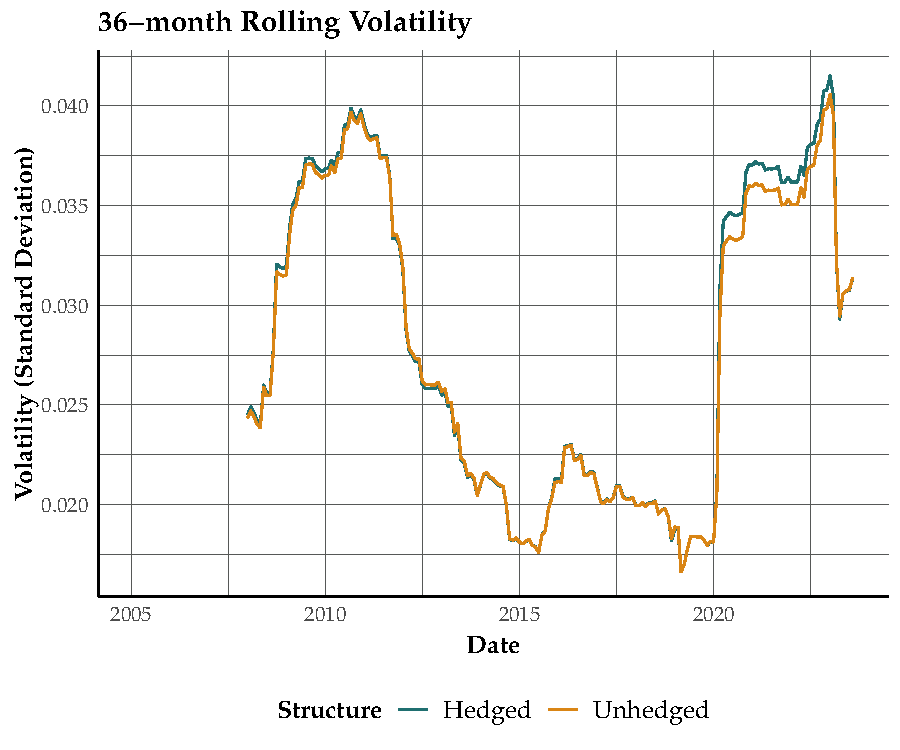
\includegraphics{Question-2_files/figure-latex/rolling-ret-1.pdf}

The figure above presents a comparison of 36-month rolling volatility
between hedged and unhedged portfolio structures. The two portfolios
track closely together throughout the timeline, with the unhedged
portfolio exhibiting slightly higher volatility at various points.
Notably, both portfolios experience a sharp rise in volatility around
2020, likely reflecting the increased market uncertainty during that
period. The convergence of the two lines for most of the observed period
suggests that currency hedging may not significantly reduce portfolio
volatility over a longer time horizon.

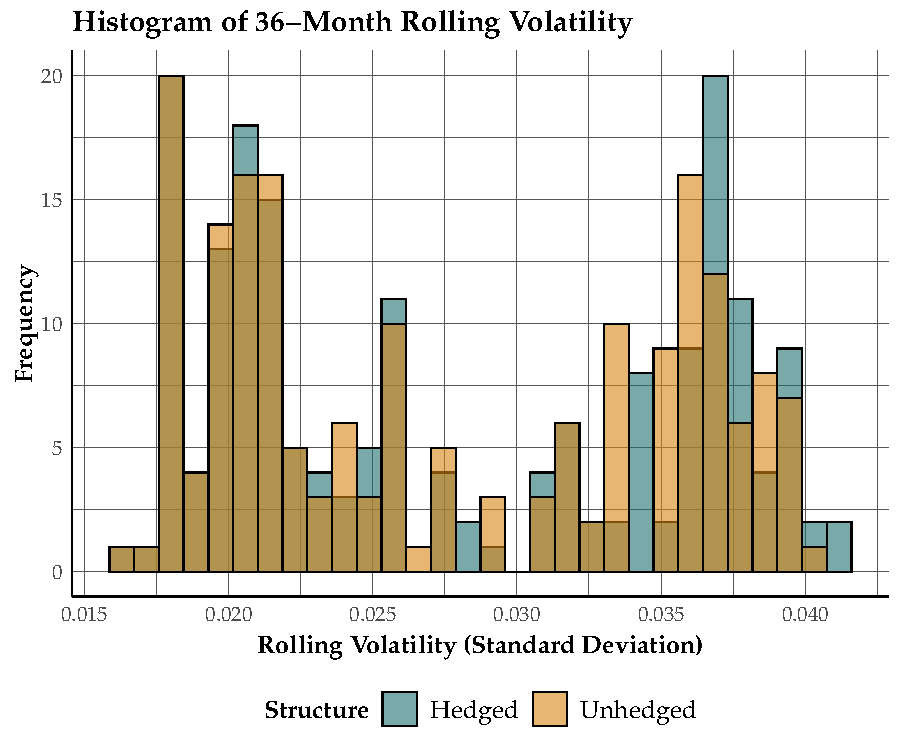
\includegraphics{Question-2_files/figure-latex/histogram-1.pdf}

The histogram above compares the distribution of 36-month rolling
volatility for hedged and unhedged portfolios. Both distributions appear
to have a similar central tendency, but the unhedged portfolio displays
a slightly wider spread, indicating more frequent occurrences of higher
volatility levels. The hedged portfolio's distribution is slightly
skewed towards lower volatility levels, suggesting that while hedging
may not drastically reduce overall volatility, it might limit the
frequency of higher volatility outcomes. Despite this, there's
considerable overlap in the volatility distributions of both strategies,
reinforcing the conclusion that the benefits of hedging in terms of
reducing volatility may be marginal.

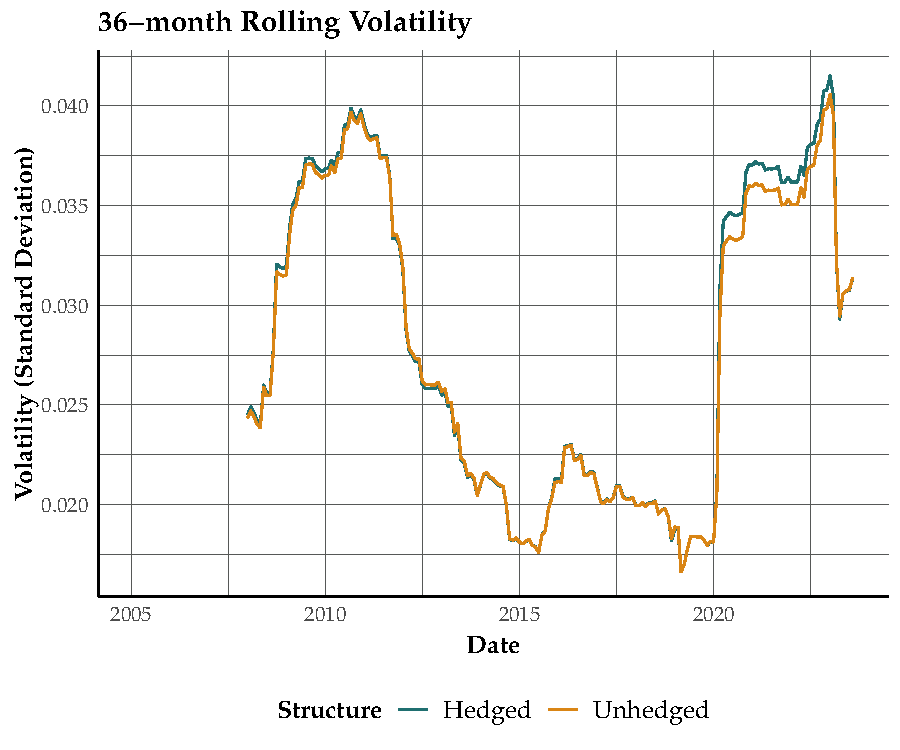
\includegraphics{Question-2_files/figure-latex/unnamed-chunk-2-1.pdf}
The Violin Plot of 36-Month Rolling Volatility indicates that both
hedged and unhedged portfolios have a similar central volatility
frequency, but the unhedged portfolio exhibits a slightly wider
distribution, suggesting more frequent high volatility occurrences. The
symmetry of both distributions implies a balanced spread of volatility
around the median, and the presence of outliers shows that extreme
values were present in both portfolios, though marginally more
pronounced in the unhedged portfolio. Overall, the plot suggests that
while hedging might slightly constrain volatility, both strategies
experience a comparable range of volatility over the long term.

\hypertarget{conclusion}{%
\section{Conclusion}\label{conclusion}}

The results demonstrate that the decision to hedge a portfolio does not
consistently lead to significant differences in performance or risk
metrics over time. The cumulative and rolling returns, alongside the
scatter plot analysis, suggest that hedging's influence is nuanced, with
periods of outperformance and underperformance that tend to cancel each
other out in the long run. Furthermore, volatility assessments,
encompassing downside risk measures and the distribution of rolling
volatilities, reveal that hedging may slightly reduce the frequency of
high volatility instances without drastically altering the overall
risk-return profile. These findings highlight the importance of aligning
hedging strategies with an investor's specific objectives and risk
appetite, rather than a one-size-fits-all approach, as the benefits of
hedging appear to be context-dependent and marginal when viewed through
the lens of an extended investment timeline.

\bibliography{Tex/ref}





\end{document}
